\documentclass[11pt]{article}

% ---------- packages ----------
\usepackage[margin=1in]{geometry}
\usepackage{amsmath, amssymb, amsthm}
\usepackage{graphicx}      % figures
\usepackage{booktabs}      % nice tables
\usepackage{enumitem}      % control over (a), (b), ...
\usepackage{siunitx}       % \num{} for consistent sig figs
\usepackage{xcolor}        % only for the \todo markers below -- delete when done
\usepackage[colorlinks=true, urlcolor=blue]{hyperref}

% ---------- shortcuts ----------

\sisetup{round-mode=figures, round-precision=4}

\title{Markov Processes --- Homework 2}
\author{Linden Kurtz}
\date{Due September 9, 2026}

\begin{document}
\maketitle

\noindent
GitHub account: \texttt{lindenkurtz} \\
Repository: \url{https://github.com/lindenkurtz/Markov2026}

\section*{Problem 1: Discrete inverse transform}

\begin{enumerate}[label=(\alph*)]
    \item
    Since we're given that the pmf of $Z$ can be described by
    \[
        p(Z) = \begin{cases}
            0.05 & \text{if } z = 1 \\
            0.15 & \text{if } z = 2 \\
            0.80 & \text{if } z = 3 \\
            0    & \text{otherwise}
        \end{cases}
    \]
    It follows that the cdf is given by
    \[
        F(z) = \begin{cases}
            0    & \text{if } z < 1 \\
            0.05 & \text{if } 1 \le z < 2 \\
            0.20 & \text{if } 2 \le z < 3 \\
            1    & \text{if } z \ge 3
        \end{cases}
    \]
    So, to sample $Z$, assuming $U \sim \operatorname{Uniform}(0, 1)$,
    \begin{verbatim}
        if (U < 0.05) return 1
        else if (U < 0.20) return 2
        else return 3
    \end{verbatim}

    \item 
    If we take $I$ to be an random variable that represents the number of inequalities checked,
    \[
        \mathbb{E}[I] = 0.05*1 + 0.95*2 = 1.95
    \]
    To minimize this value, we could instead check the most likely condition first, then move from most to least likely, such as with the pseudocode:
    \begin{verbatim}
        if (U < 0.80) return 3
        else if (U < 0.95) return 2
        else return 1
    \end{verbatim}
    Which results in the expected value
    \[
        \mathbb{E}[I] = 0.80*1 + 0.20*2 = 1.2
    \]

    \item 
    Given that $X \sim \operatorname{Geometric}(p)$, solving for $F(k) \ge U$ gives:
    \begin{align*}
        1-(1-p)^k &\ge U \\
        k &\ge \log_{1-p} (1-U) \\
        k &\ge \frac{\ln(1-U)}{\ln(1-p)} \\
    \end{align*}
    Since $X$ is the smallest such $k$, and $k$ must be a positive integer,
    \[
        X = \left\lceil\frac{\ln(1-U)}{\ln(1-p)}\right\rceil
    \]

\end{enumerate}

\section*{Problem 2: Inverse transform on the whole line}

\begin{enumerate}[label=(\alph*)]
    \item
    The standard Cauchy density is $f(x) = \dfrac{1}{\pi(1+x^2)}$ for $x \in \mathbb{R}$, so the cdf
    is
    \begin{align*}
        F(x) &= \int_{-\infty}^{x} f(y) \, dy = \frac{1}{\pi}\int_{-\infty}^{x} \frac{1}{1+y^2} \, dy, \\
             &= \frac{1}{\pi}\left(\arctan y \right)\Big|_{-\infty}^{x}, \\
             &= \frac{1}{\pi}\left(\arctan x + \frac{\pi}{2}\right), \\
             &= \frac{1}{2} + \frac{1}{\pi}\arctan x
    \end{align*}
    To invert, set $x = \frac{1}{2} + \frac{1}{\pi}\arctan\!\left(F^{-1}(x)\right)$ and solve:
    \begin{align*}
        \arctan\!\left(F^{-1}(x)\right) &= \pi\left(x - \frac{1}{2}\right), \\
        F^{-1}(x) &= \tan\!\left(\pi x - \frac{\pi}{2}\right)
    \end{align*}
    So, assuming $U \sim \operatorname{Uniform}(0, 1)$,
    \begin{verbatim}
        U = rand(0, 1)
        X = tan(pi*U - pi/2)
    \end{verbatim}

    \item
    For the median $m$ of $|X|$, we need $\mathbb{P}(|X| \le m) = 0.5$. Since the Cauchy density is
    symmetric about zero,
    \begin{align*}
        0.5 &= \mathbb{P}(|X| \le m) = \mathbb{P}(-m \le X \le m), \\
            &= F(m) - F(-m), \\
            &= \frac{1}{2} + \frac{1}{\pi}\arctan(m) - \frac{1}{2} - \frac{1}{\pi}\arctan(-m), \\
            &= \frac{1}{\pi}\left(\arctan(m) - \arctan(-m)\right), \\
            &= \frac{2}{\pi}\arctan(m)
    \end{align*}
    so $\arctan(m) = \frac{\pi}{4}$ and $m = \tan\!\left(\frac{\pi}{4}\right) = 1$. \\ \\
    For the mean, substituting $u = 1 + x^2$ so that $du = 2x \, dx$ and $\frac{1}{2} du = x \, dx$,
    \begin{align*}
        \mathbb{E}|X| &= \int_{-\infty}^{\infty} |x| f(x) \, dx
                       = \frac{1}{\pi}\int_{-\infty}^{\infty} \frac{|x|}{1+x^2} \, dx, \\
                      &= \frac{1}{\pi}\int_{-\infty}^{0} \frac{-x}{1+x^2} \, dx
                       + \frac{1}{\pi}\int_{0}^{\infty} \frac{x}{1+x^2} \, dx, \\
                      &= \frac{1}{\pi}\int_{\infty}^{1} \frac{-1}{2u} \, du
                       + \frac{1}{\pi}\int_{1}^{\infty} \frac{1}{2u} \, du, \\
                      &= \frac{-1}{2\pi}\left(\ln|u|\right)\Big|_{\infty}^{1}
                       + \frac{1}{2\pi}\left(\ln|u|\right)\Big|_{1}^{\infty}, \\
                      &= \frac{-1}{2\pi}\left(0 - \infty\right) + \frac{1}{2\pi}\left(\infty - 0\right)
                       = \infty
    \end{align*}
    If a distribution contains a low likelihood of very large values (i.e.\ the values grow faster
    than the tail shrinks), its expected value can increase toward $\infty$ while $50\%$ of draws are
    still below a finite value.
\end{enumerate}

\section*{Problem 3: Acceptance--rejection with an exponential envelope}

\begin{enumerate}[label=(\alph*)]
    \item
    We want the smallest $c$ with $f(x) \le c\,g(x)$ for all $x \ge 0$, which is
    $c = \max_{x \ge 0} f(x)/g(x)$. With $\lambda = \frac{1}{2}$,
    \[
        \frac{f(x)}{g(x)} = \frac{x e^{-x}}{\frac{1}{2}e^{-x/2}} = 2x e^{-x/2}
    \]
    Differentiating and setting equal to zero,
    \begin{align*}
        2\left(-\frac{1}{2} x e^{-x/2} + e^{-x/2}\right) &= 0, \\
        2e^{-x/2}\left(-\frac{x}{2} + 1\right) &= 0, \\
        x &= 2
    \end{align*}
    so the maximum is at $x = 2$ and
    \[
        c = 2\left(2e^{-1}\right) = \frac{4}{e} \approx \num{1.4715}
    \]
    For the theoretical acceptance rate, $\int_{-\infty}^{\infty} f(x) \, dx = 1$ while
    $\int_{-\infty}^{\infty} c\,g(x) \, dx = c$, so
    \[
        \mathbb{P}(\text{accept}) = \frac{1}{c} = \frac{e}{4} \approx \num{0.6796}
    \]
    Finally, the acceptance test $U < \dfrac{f(X)}{c\,g(X)}$ simplifies to
    \begin{align*}
        U &< \frac{X e^{-X}}{\left(\frac{4}{e}\right)\left(\frac{1}{2}\right)e^{-X/2}}
           = \frac{e \cdot X \cdot e^{-X/2}}{2}, \\
        U &< \left(\frac{e}{2}\right) X e^{-X/2}
    \end{align*}

    \item
    Sampling the proposal by inversion, $G(x) = 1 - e^{-x/2}$ gives
    \begin{align*}
        x &= 1 - e^{-G^{-1}(x)/2}, \\
        -x + 1 &= e^{-G^{-1}(x)/2}, \\
        G^{-1}(x) &= -2\ln(1-x)
    \end{align*}
    so the sampler is
    \begin{verbatim}
        while (true):
            U1 = rand(0, 1)
            U2 = rand(0, 1)
            X = -2 * ln(1 - U1)
            if (U2 < (e/2) * X * exp(-X/2)):
                break
        return X
    \end{verbatim}

    \item
    Implemented in \texttt{problem\_3.py} for $N = 10^4$ accepted samples at
    $\lambda = \frac{1}{2}$ and $\lambda = 0.2$.

    \begin{table}[ht]
        \centering
        \begin{tabular}{lcccc}
            \toprule
            $\lambda$ & $c$ & $1/c$ & empirical acceptance & time per accepted sample \\
            \midrule
            $1/2$ & $\num{1.4715}$ & $\num{0.6796}$ & $\num{0.6804}$ & $1.0\,\mu$s \\
            $0.2$ & $\num{2.2992}$ & $\num{0.4349}$ & $\num{0.4324}$ & $1.5\,\mu$s \\
            \bottomrule
        \end{tabular}
    \end{table}

    \begin{figure}[ht]
        \centering
        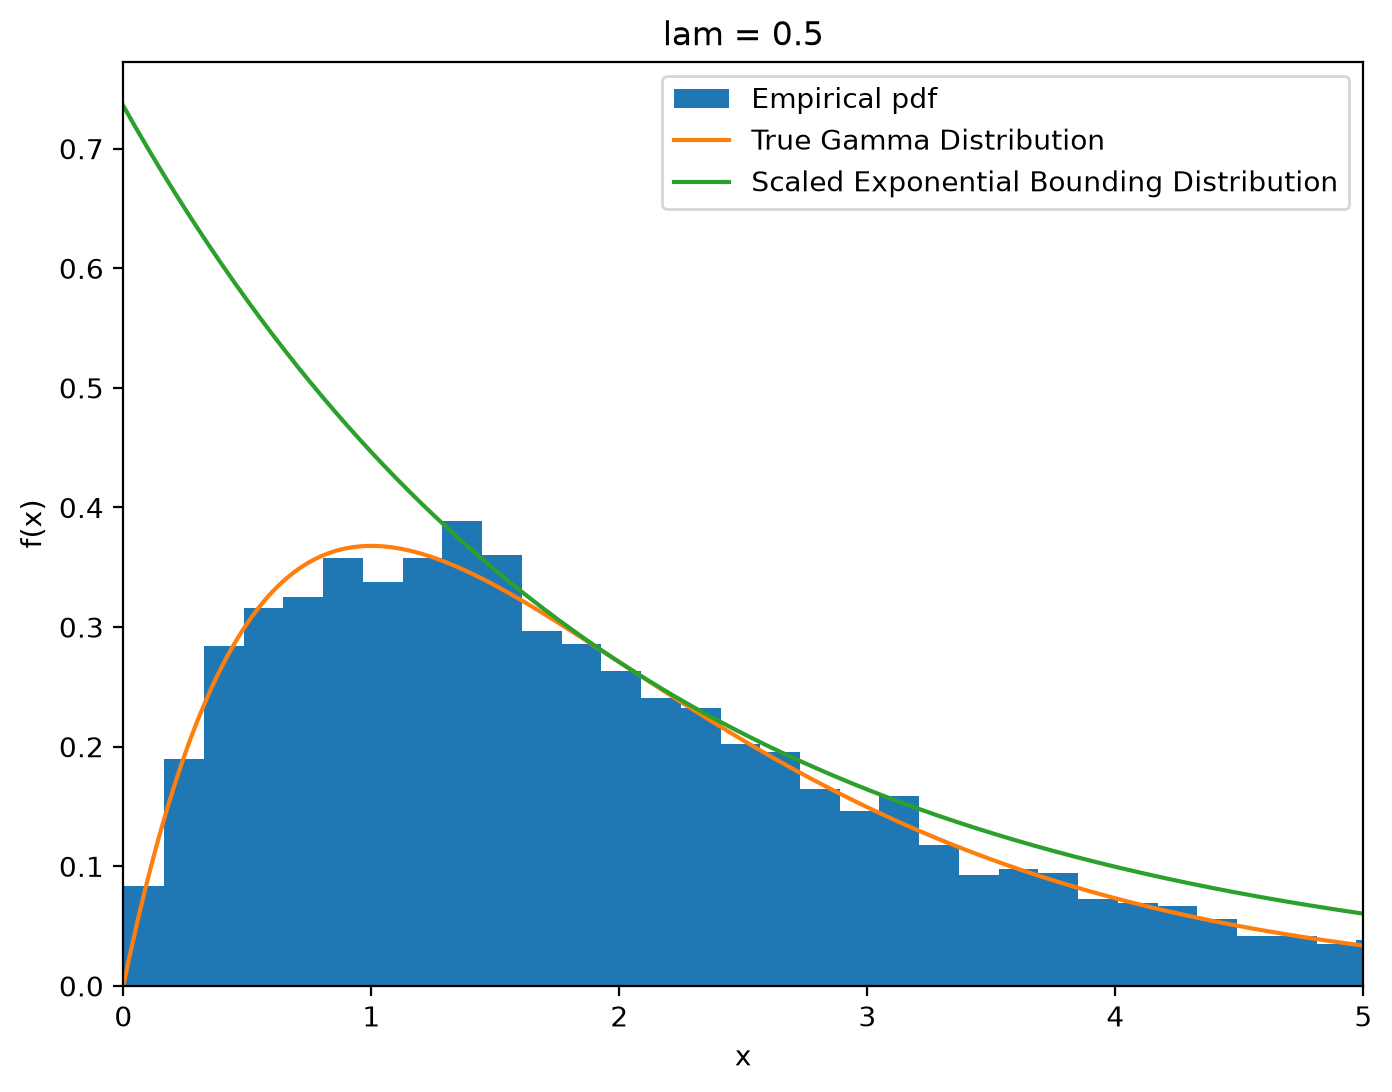
\includegraphics[width=0.72\textwidth]{problem_3_lam=0.5.png}
        \caption{$\lambda = 1/2$: normalized histogram of $10^4$ accepted samples with $f(x)$ and the
        envelope $c\,g(x)$ overlaid. Bin width = 0.1603}
    \end{figure}

    \begin{figure}[ht]
        \centering
        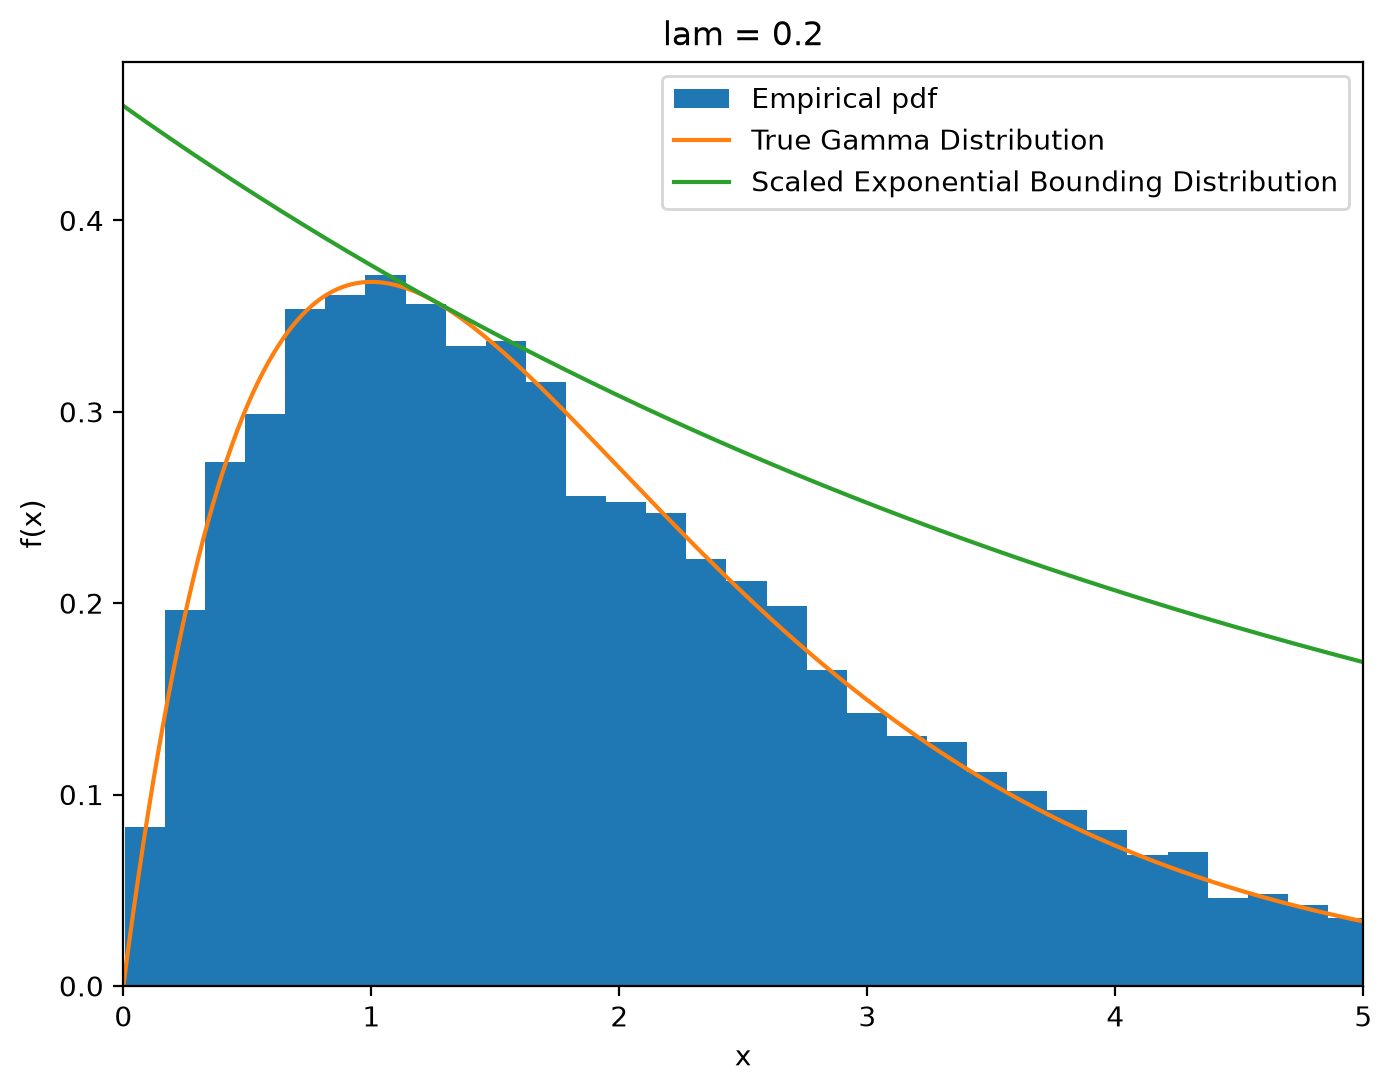
\includegraphics[width=0.72\textwidth]{problem_3_lam=0.2.png}
        \caption{$\lambda = 0.2$: normalized histogram of $10^4$ accepted samples with $f(x)$ and the
        envelope $c\,g(x)$ overlaid. Bin width = 0.1617}
    \end{figure}

    When \(\lambda = 0.5\), the empirical acceptence is higher and the time per accepted sample is
    lower, which makes sense because less loops are happening per sample, on average. with \(\lambda = 0.2\), 
    the empirical acceptance is lower and the time per accepted sample is
    higher, since more iterations are being spent per accept-reject loop.

\end{enumerate}

\penalty-10000

\section*{Problem 4: Ion channel dwell times and mixture sampling}

Throughout, $a = 0.9$, $\lambda_f = 1000\ \mathrm{s}^{-1}$ and $\lambda_s = 10\ \mathrm{s}^{-1}$.

\begin{enumerate}[label=(\alph*)]
    \item
    The density is a sum of two nonnegative terms, so $f(t) \ge 0$ for $t \ge 0$, and it integrates
    to one:
    \begin{align*}
        \int_{-\infty}^{\infty} f(t) \, dt
        &= \int_{0}^{\infty} a\lambda_f e^{-\lambda_f t} + (1-a)\lambda_s e^{-\lambda_s t} \, dt, \\
        &= a\lambda_f \int_{0}^{\infty} e^{-\lambda_f t} \, dt
         + (1-a)\lambda_s \int_{0}^{\infty} e^{-\lambda_s t} \, dt, \\
        &= a\lambda_f\left(\frac{-1}{\lambda_f}e^{-\lambda_f t}\Big|_{0}^{\infty}\right)
         + (1-a)\lambda_s\left(\frac{-1}{\lambda_s}e^{-\lambda_s t}\Big|_{0}^{\infty}\right), \\
        &= a + (1-a) = 1
    \end{align*}
    so $f$ is a valid pdf. For the moments, each integral is the corresponding moment of an
    exponential, so
    \begin{align*}
        \mathbb{E}[T] &= \int_{0}^{\infty} t f(t) \, dt
        = a \int_{0}^{\infty} t \lambda_f e^{-\lambda_f t} \, dt
        + (1-a) \int_{0}^{\infty} t \lambda_s e^{-\lambda_s t} \, dt, \\
        &= a \cdot \frac{1}{\lambda_f} + (1-a) \cdot \frac{1}{\lambda_s}
         = \frac{a}{\lambda_f} + \frac{1-a}{\lambda_s} = \num{0.0109}\ \mathrm{s}
    \end{align*}
    and, using $\mathbb{E}[X^2] = 2/\lambda^2$ for an exponential,
    \begin{align*}
        \mathbb{E}[T^2] &= a \cdot \frac{2}{\lambda_f^2} + (1-a) \cdot \frac{2}{\lambda_s^2}, \\
        \operatorname{Var}(T) &= \mathbb{E}[T^2] - \mathbb{E}[T]^2
        = \frac{2a}{\lambda_f^2} + \frac{2(1-a)}{\lambda_s^2}
          - \left(\frac{a}{\lambda_f} + \frac{1-a}{\lambda_s}\right)^2, \\
        &= \frac{a(2-a)}{\lambda_f^2} - \frac{2a(1-a)}{\lambda_f \lambda_s}
         + \frac{(1-a)\left(2-(1-a)\right)}{\lambda_s^2}
         = \num{0.0018830}\ \mathrm{s}^2
    \end{align*}
    Putting both over a common denominator, the coefficient of variation is
    \begin{align*}
        \mathrm{CV} &= \frac{\sqrt{\operatorname{Var}(T)}}{\mathbb{E}[T]}
        = \frac{\sqrt{\dfrac{\lambda_s^2 a(2-a) - 2\lambda_f\lambda_s a(1-a)
            + \lambda_f^2 (1-a)\left(2-(1-a)\right)}{\lambda_f^2 \lambda_s^2}}}
          {\dfrac{a\lambda_s + (1-a)\lambda_f}{\lambda_f \lambda_s}}, \\
        &= \frac{\sqrt{\lambda_s^2 a(2-a) - 2\lambda_f\lambda_s a(1-a) + \lambda_f^2 (1-a^2)}}
                {a\lambda_s + (1-a)\lambda_f}
        \approx \num{3.981}
    \end{align*}
    For a single exponential,
    \[
        \mathrm{CV} = \frac{\sqrt{\frac{1}{\lambda^2}}}{\frac{1}{\lambda}} = 1
    \]
    This means the standard deviation as a proportion of the mean is larger for $T$ than for an
    exponential distribution. In other words, $T$ is effectively more random than an exponential.

    \item
    Each component is exponential with cdf $F(t) = 1 - e^{-\lambda t}$, so
    \begin{align*}
        t &= 1 - e^{-\lambda F^{-1}(t)}, \\
        e^{-\lambda F^{-1}(t)} &= 1 - t, \\
        -\lambda F^{-1}(t) &= \ln|1-t|, \\
        F^{-1}(t) &= \frac{-\ln(1-t)}{\lambda}
    \end{align*}
    The composition algorithm draws one Bernoulli variate to pick the component and one uniform to
    invert it:
    \begin{verbatim}
        U1 = rand(0, 1)
        U2 = rand(0, 1)
        if (U1 <= a):
            X = -ln(1 - U2) / lambda_f
        else:
            X = -ln(1 - U2) / lambda_s
    \end{verbatim}

    \item
    Implemented in \texttt{problem\_4.py} for $N = 10^5$ dwell times.

    \begin{figure}[ht]
        \centering
        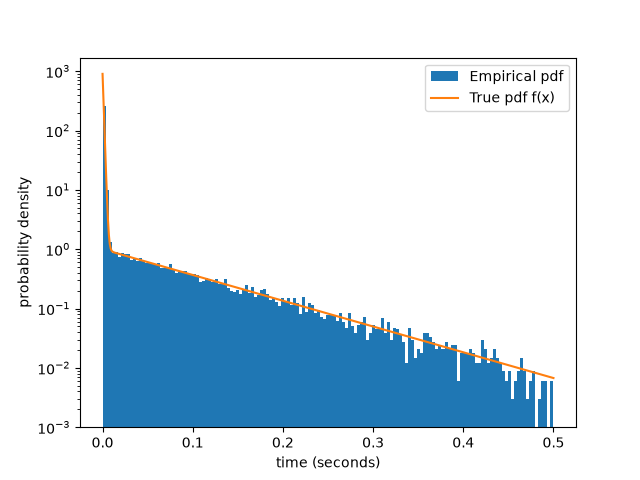
\includegraphics[width=0.72\textwidth]{problem_4.png}
        \caption{Normalized histogram of $10^5$ closed dwell times with $f(t)$ overlaid, semilog
        vertical axis. Bin width = 3.356}
    \end{figure}

    \begin{table}[ht]
        \centering
        \begin{tabular}{lccc}
            \toprule
            theoretical \(\mathbb{E}[T]\) & empirical \(\mathbb{E}[T]\) & theoretical $\mathbb{P}(T > 50\ \mathrm{ms})$ & empirical $\mathbb{P}(T > 50\ \mathrm{ms})$ \\
            \midrule
            $\num{0.01090}$ & $\num{0.01079}$ & $\num{0.06065}$ & $\num{0.06039}$ \\
            \bottomrule
        \end{tabular}
    \end{table}
    Where the theoretical tail probability is
    \[
        \mathbb{P}(T > 0.05) = 1 - F(T) = a e^{-\lambda_f (0.05)} + (1-a) e^{-\lambda_s (0.05)}
        = 0.9 e^{-50} + 0.1 e^{-0.5} \approx \num{0.060653}
    \]
\end{enumerate}

\section*{Problem 5: Simulation Assignment: growth by redirection}

The process is
\[
    C(N+1) = \begin{cases}
        C(N) + 1 & \text{with probability } \mu\,C(N)/N \\
        C(N)     & \text{otherwise}
    \end{cases}
    \qquad C(3) = 1
\]
and at $\mu = 1$ the ratio $z = C(N)/N$ has limiting density $h(z) = 2(1-z)$ for $0 < z < 1$.

\begin{enumerate}[label=(\alph*)]
    \item
    The density is nonnegative on $(0,1)$ and integrates to one:
    \[
        \int_{-\infty}^{\infty} h(z) \, dz = \int_{0}^{1} 2(1-z) \, dz = \int_{0}^{1} 2 - 2z \, dz
        = \left(2z - z^2\right)\Big|_{0}^{1} = (2 - 1) - 0 = 1
    \]
    For the moments,
    \begin{align*}
        \mathbb{E}[z] &= \int_{-\infty}^{\infty} z\,h(z) \, dz = \int_{0}^{1} 2z - 2z^2 \, dz
        = \left(z^2 - \frac{2}{3}z^3\right)\Big|_{0}^{1} = 1 - \frac{2}{3} = \frac{1}{3}, \\
        \mathbb{E}[z^2] &= \int_{0}^{1} 2z^2 - 2z^3 \, dz
        = \left(\frac{2}{3}z^3 - \frac{1}{2}z^4\right)\Big|_{0}^{1} = \frac{1}{6}, \\
        \operatorname{Var}(z) &= \frac{1}{6} - \left(\frac{1}{3}\right)^2 = \frac{1}{18}
    \end{align*}
    so the ratio of standard deviation to mean is
    \[
        \frac{\sqrt{\operatorname{Var}(z)}}{\mathbb{E}[z]} = \frac{\sqrt{1/18}}{1/3}
        = \frac{1}{\sqrt{2}} \approx \num{0.7071}
    \]

    \item
    The cdf is
    \[
        H(z) = \int_{0}^{z} 2 - 2x \, dx = 2z - z^2
    \]
    To invert, write $z = 2H^{-1}(z) - \left(H^{-1}(z)\right)^2$ and complete the square:
    \begin{align*}
        z &= -\left(\left(H^{-1}(z)\right)^2 - 2H^{-1}(z)\right), \\
        z - 1 &= -\left(H^{-1}(z) - 1\right)^2, \\
        1 - z &= \left(H^{-1}(z) - 1\right)^2, \\
        H^{-1}(z) &= \pm\sqrt{1-z} + 1
    \end{align*}
    Since $+\sqrt{1-z} + 1 > 1$ falls outside the support, we take the negative root, giving
    $H^{-1}(z) = 1 - \sqrt{1-z}$ and the sampler
    \begin{verbatim}
        U = rand(0, 1)
        Z = 1 - sqrt(1 - U)
    \end{verbatim}
    Over $10^5$ samples this gives a sample mean of $\num{0.33218}$ against the theoretical
    $\mathbb{E}[z] = \frac{1}{3} \approx \num{0.33333}$ from part (a).

    \item
    Implemented in \texttt{problem\_5.py}, simulating out to $N = 10^4$ for $R = 10^3$ independent
    realizations.

    \begin{figure}[ht]
        \centering
        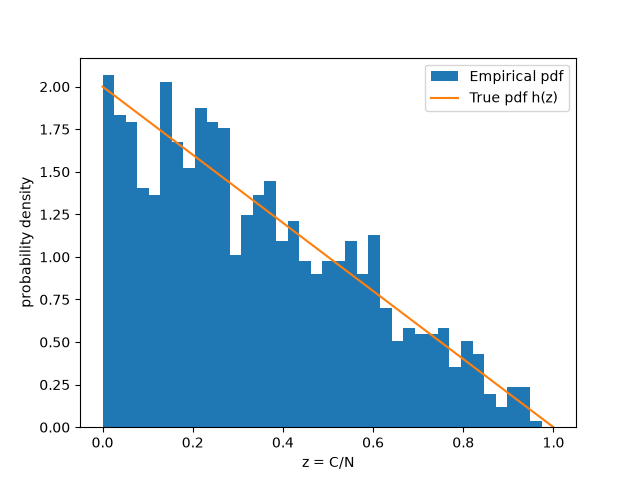
\includegraphics[width=0.72\textwidth]{problem_5.png}
        \caption{Normalized histogram of $z = C/N$ over $10^3$ realizations at $N = 10^4$, with
        $h(z) = 2(1-z)$ overlaid. Bin width = 0.02564}
    \end{figure}

    \penalty-10000

    So,
    \begin{table}[ht]
        \centering
        \begin{tabular}{lccc}
            \toprule
            theoretical mean & empirical mean & theoretical sd/mean & empirical sd/mean \\
            \midrule
            $\frac{1}{3}$ & $\num{0.33714}$ & $\frac{1}{\sqrt{2}}$ & $\num{0.69691}$ \\
            \bottomrule
        \end{tabular}
    \end{table}

    The smallest core seen across the $10^3$ realizations was $1$ and the largest was $\num{9522}$.

    While the average \(C/N\) is $\frac{1}{3}$, the sd/mean and graph show that these core sizes vary widly.
    So, the average core size can tell you how much the cores grew averaged across all realizations, but it isn't a great
    meaure of the typical network size.

\end{enumerate}

\end{document}
